%*******10********20********30********40********50********60********70********80
\clearpage
\section{Cracking Pattern caused by Pure ASR Expansion}

%*******10********20********30********40********50********60********70********80

\subsection{Single ASR Expansion Simulation}

%*******10********20********30********40********50********60********70********80
% illustration of A30P75 ASR C D0 A0.001 S20 Expansion

In this section, the process of simulated one ASR expansion is present. The expanse is generated at the location of interfaces between mortar and reactive aggregate, to introduce the expansion, as introduced in chapter 2.

For usually the case not all aggregate inside concrete structure are ASR reactive aggregate, here only partial of aggregates are selected to be ASR reactive and will be givin initial strain in expansion steps to simulate ASR expansion.

This single example case has been choosing here use the model in the dimension of 100x100x100mm, with 30\% aggregate, of which 75\% are ASR reactive. Aggregate in Figure \ref{fig:A30_model} in red color is assumed as ASR reactive, while aggregate in blue color is assumed as non-reactive aggregate.

  \begin{figure}[ht!]
  \centering
  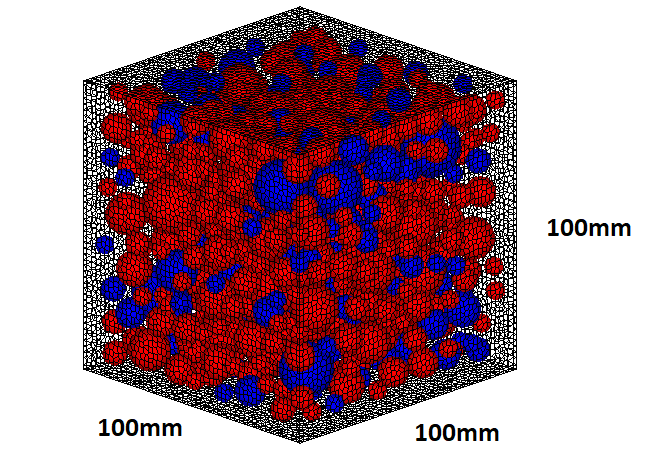
\includegraphics[width=.3\linewidth]{Files/Aggregate/A30P75.png}
    \caption{30\% Coarse Aggregate}
    \label{fig:A30_model}
  \end{figure}

Table. Aggregate consistent(if we have it)

To simulate ASR expansion, an initial strain of 0.001mm is given in each step, for totally 20 steps expansion. Before and after expansion, the distance of element between 2 elements is recorded to gauge the gloal expansion. These two element selected here are the middle element in the left surface of model and the middle element in the left surface of model.

% TODO: A30 illustration d between 113942 116197

%*******10********20********30********40********50********60********70********80

% illustration of A30P75 ASR C D0 A0.001 S20 Expansion

  \begin{table}[ht]
  \centering
  \begin{tabular}{ ||p{3cm}|p{3cm}||p{3cm}|p{3cm}|| }
  \hline
   Step &  Expansion & Step & Expansion \\
   \hline\hline
    1 & 0.000136  & 11 & 0.002140 \\
    2 & 0.000314  & 12 & 0.002358 \\
    3 & 0.000501  & 13 & 0.002582 \\
    4 & 0.000695  & 14 & 0.002812 \\
    5 & 0.000894  & 15 & 0.003049 \\
    6 & 0.001096  & 16 & 0.003278 \\
    7 & 0.001301  & 17 & 0.003536 \\
    8 & 0.001507  & 18 & 0.003767 \\
    9 & 0.001715  & 19 & 0.003989 \\
    10 & 0.001924  & 20  & 0.004223 \\
    \hline
    \end{tabular}
  \caption{Expansion in Each Step for A30 P75 Case 3}
  \label{table:A30P75_3_EXP}
  \end{table}

  \begin{figure}[ht!]
  \centering
  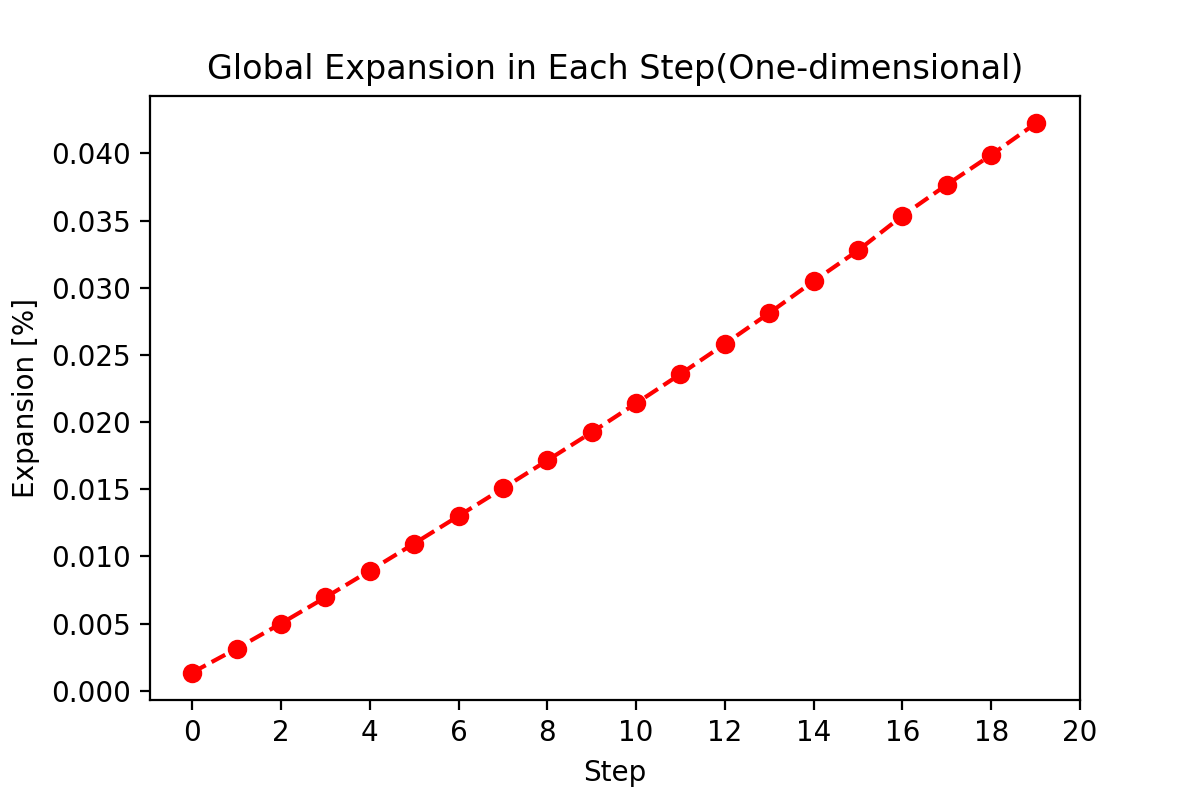
\includegraphics[width=.8\linewidth]{Files/exp_plot/ASRA30P75_3_exp.png}
    \caption{Global Expansion vs. Step}
    \label{fig:ASRA30P75_3_exp}
  \end{figure}

%*******10********20********30********40********50********60********70********80

With the increasing of initial strain giving, the global expansion also gradually increasing. After 20 steps of ASR expansion, the model here reached 0.4223\% expansion(one-dimensionally). Characteristic ASR map cracking pattern can be seen on the surface of the expanded concrete model in Figure \ref{fig:ASR_A30P75_3_3D_1}.

Here the surface cracking from experimental result, done by ALKANA in 2013, is shown in Figure \ref{ALKANASRcrack}, in shape of 100x100x400mm, with 0.10 percent one-dimensional expansion. It can be seen that in Figure \ref{fig:ASR_A30P75_3_3D_1}, similar map cracking is represented.

  \begin{figure}[ht!]
  \centering
  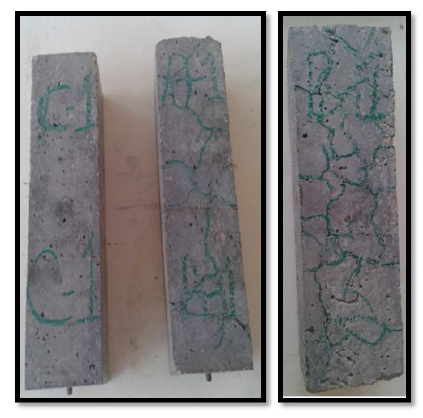
\includegraphics[width=.8\linewidth]{Reference/ALKANASRcrack.png}
    \caption{Prismatic specimens of G-C, G-A, and G-B concretes respectively[ALKANA, 2012]}
    \label{ALKANASRcrack}
  \end{figure}


% ASRA30P75_3 Surface Cracking
  \begin{figure}[ht]
  \centering
      %*******
      \begin{subfigure}{.5\textwidth}
        \centering
        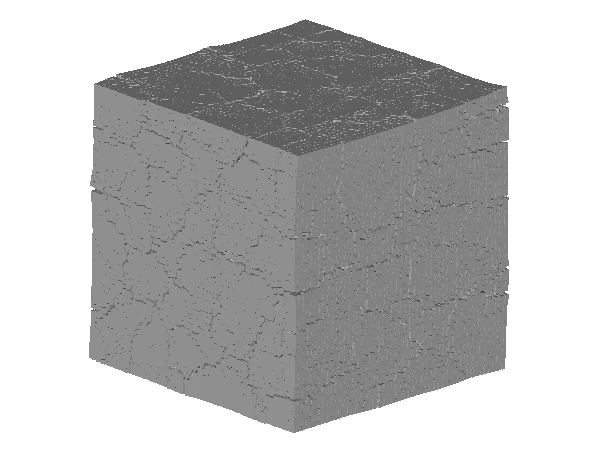
\includegraphics[width=.8\linewidth]{Files/exp_3D/ASR/A30P75_3_3d.png}
      \end{subfigure}%
      \begin{subfigure}{.5\textwidth}
        \centering
        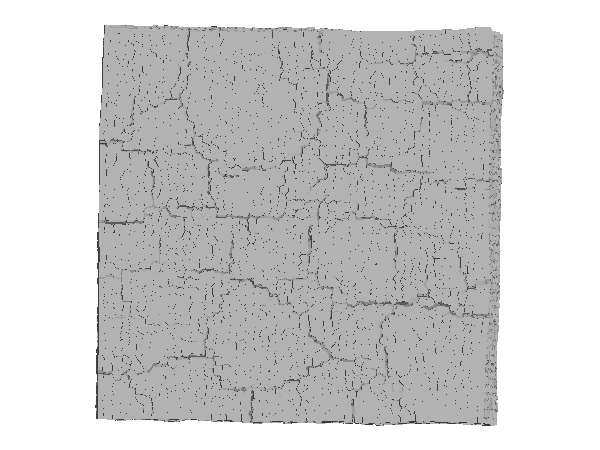
\includegraphics[width=.8\linewidth]{Files/exp_3D/ASR/A30P75_3_3ds.png}
        \end{subfigure}
        %*******
    \caption{3D Surface Cracks, 0.4223\% Expansion (Deformation x 10)}
    \label{fig:ASR_A30P75_3_3D_1}
  \end{figure}

% Internal Stress for step 1-20 ASR_A30_P75_3

  \begin{figure}[ht!]
  \centering
      %*******
      \begin{subfigure}{.25\textwidth}
        \centering
        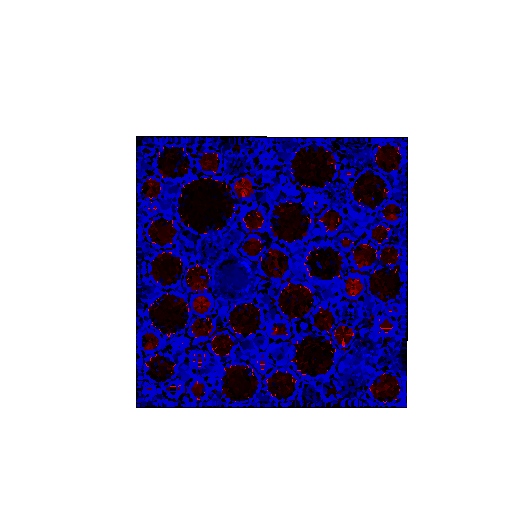
\includegraphics[width=1.0\linewidth]{Files//A30P75_3_IS/DEP50-STEP(001).png}
      \caption{Step 1}
      \end{subfigure}%
      %*******
      \begin{subfigure}{.25\textwidth}
        \centering
        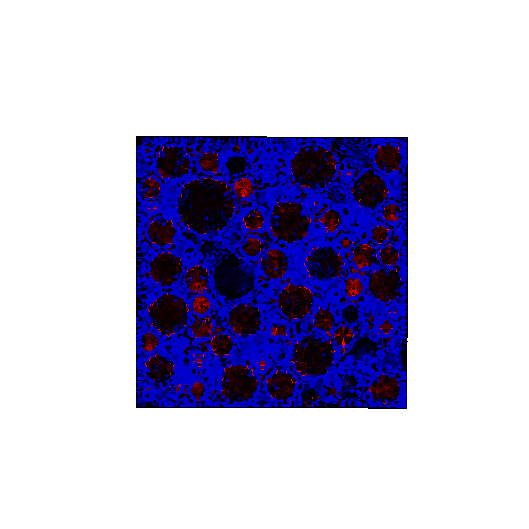
\includegraphics[width=1.0\linewidth]{Files/A30P75_3_IS/DEP50-STEP(002).png}
      \caption{Step 2}
      \end{subfigure}%
      %*******
      \begin{subfigure}{.25\textwidth}
        \centering
        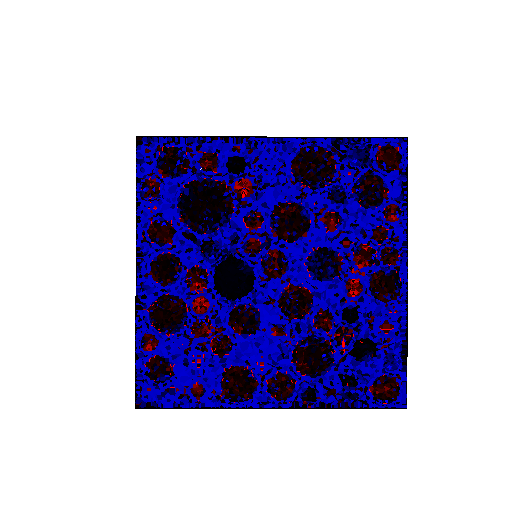
\includegraphics[width=1.0\linewidth]{Files/A30P75_3_IS/DEP50-STEP(003).png}
      \caption{Step 3}
      \end{subfigure}%
      %*******
      \begin{subfigure}{.25\textwidth}
        \centering
        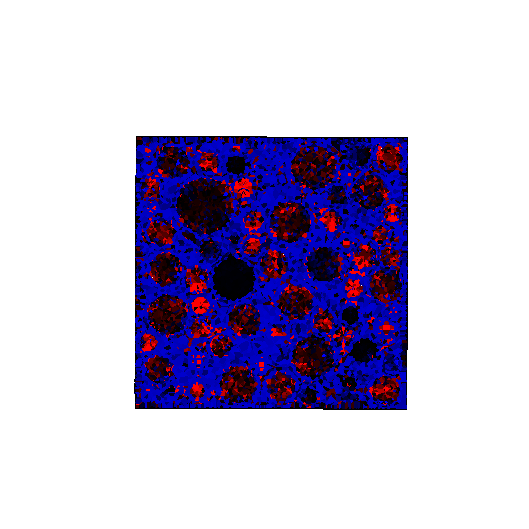
\includegraphics[width=1.0\linewidth]{Files/A30P75_3_IS/DEP50-STEP(004).png}
      \caption{Step 4}
      \end{subfigure}

      %*******
      %*******
      \begin{subfigure}{.25\textwidth}
        \centering
        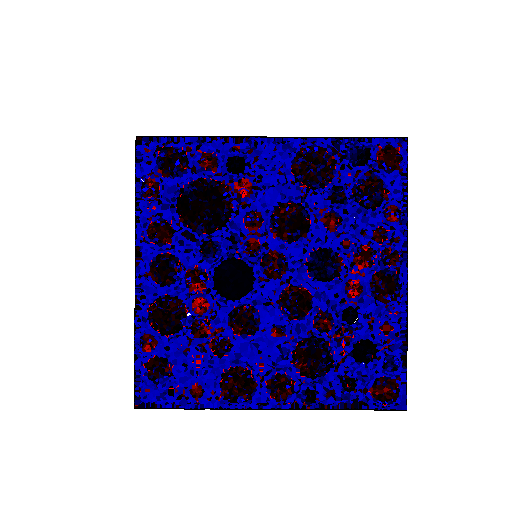
\includegraphics[width=1.0\linewidth]{Files//A30P75_3_IS/DEP50-STEP(005).png}
      \caption{Step 5}
      \end{subfigure}%
      %*******
      \begin{subfigure}{.25\textwidth}
        \centering
        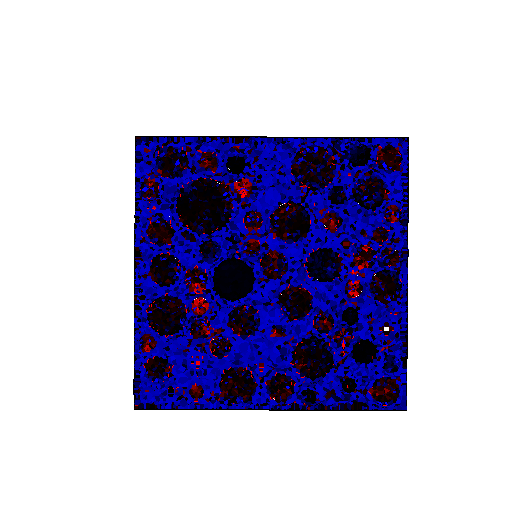
\includegraphics[width=1.0\linewidth]{Files/A30P75_3_IS/DEP50-STEP(006).png}
      \caption{Step 6}
      \end{subfigure}%
      %*******
      \begin{subfigure}{.25\textwidth}
        \centering
        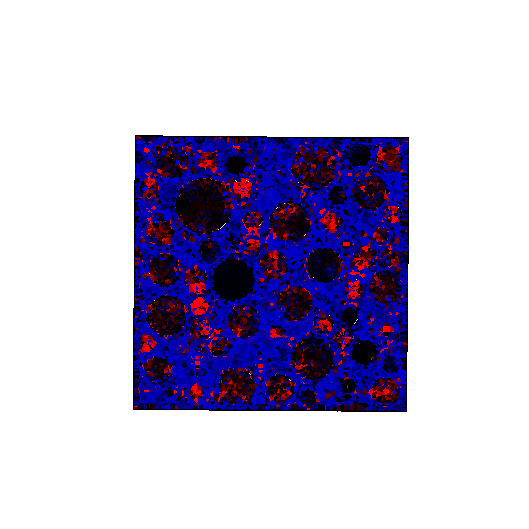
\includegraphics[width=1.0\linewidth]{Files/A30P75_3_IS/DEP50-STEP(007).png}
      \caption{Step 7}
      \end{subfigure}%
      %*******
      \begin{subfigure}{.25\textwidth}
        \centering
        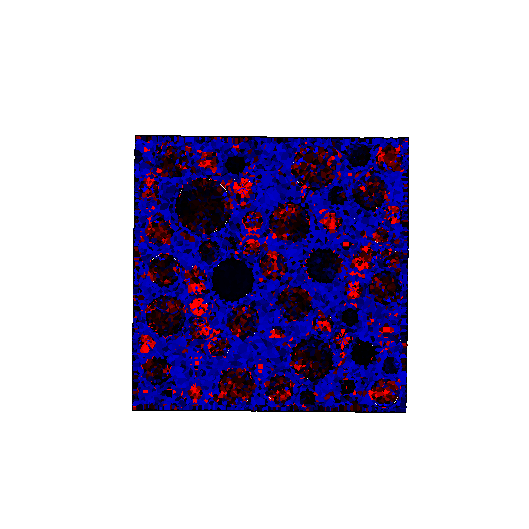
\includegraphics[width=1.0\linewidth]{Files/A30P75_3_IS/DEP50-STEP(008).png}
      \caption{Step 4}
      \end{subfigure}

      %*******
      %*******
      \begin{subfigure}{.25\textwidth}
        \centering
        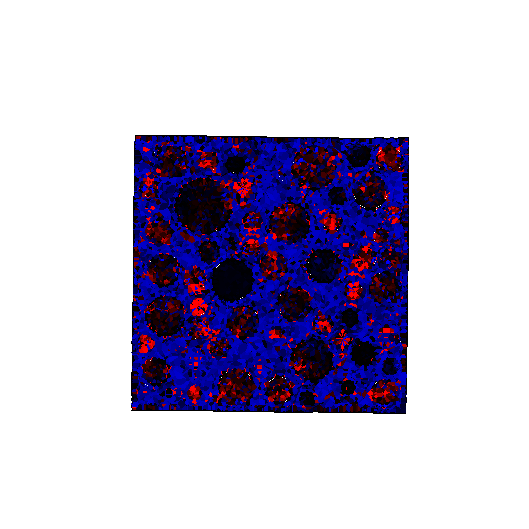
\includegraphics[width=1.0\linewidth]{Files//A30P75_3_IS/DEP50-STEP(009).png}
      \caption{Step 9}
      \end{subfigure}%
      %*******
      \begin{subfigure}{.25\textwidth}
        \centering
        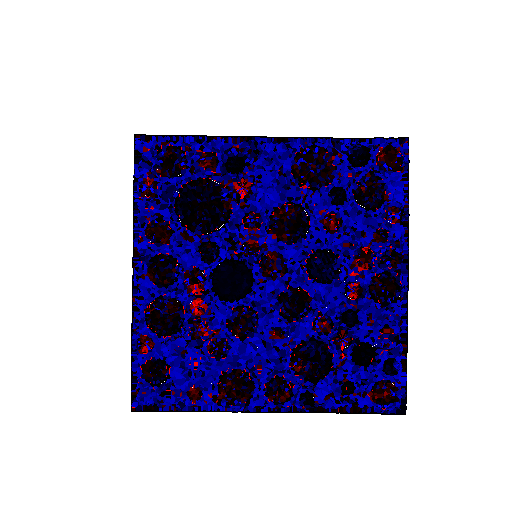
\includegraphics[width=1.0\linewidth]{Files/A30P75_3_IS/DEP50-STEP(010).png}
      \caption{Step 10}
      \end{subfigure}%
      %*******
      \begin{subfigure}{.25\textwidth}
        \centering
        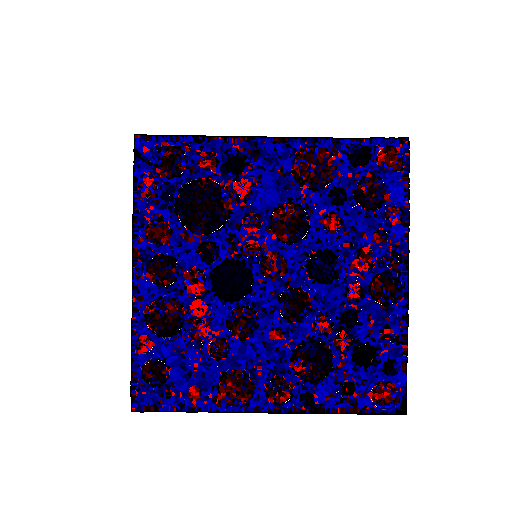
\includegraphics[width=1.0\linewidth]{Files/A30P75_3_IS/DEP50-STEP(011).png}
      \caption{Step 11}
      \end{subfigure}%
      %*******
      \begin{subfigure}{.25\textwidth}
        \centering
        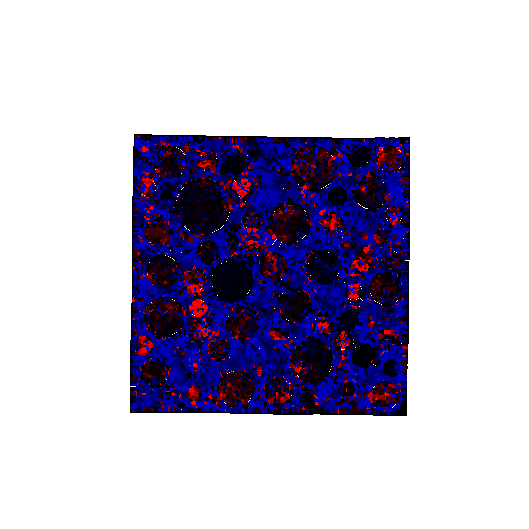
\includegraphics[width=1.0\linewidth]{Files/A30P75_3_IS/DEP50-STEP(012).png}
      \caption{Step 12}
      \end{subfigure}

      %*******
      %*******
      \begin{subfigure}{.25\textwidth}
        \centering
        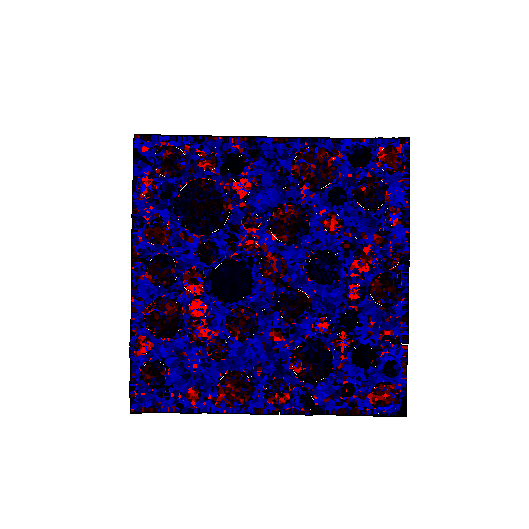
\includegraphics[width=1.0\linewidth]{Files//A30P75_3_IS/DEP50-STEP(013).png}
      \caption{Step 13}
      \end{subfigure}%
      %*******
      \begin{subfigure}{.25\textwidth}
        \centering
        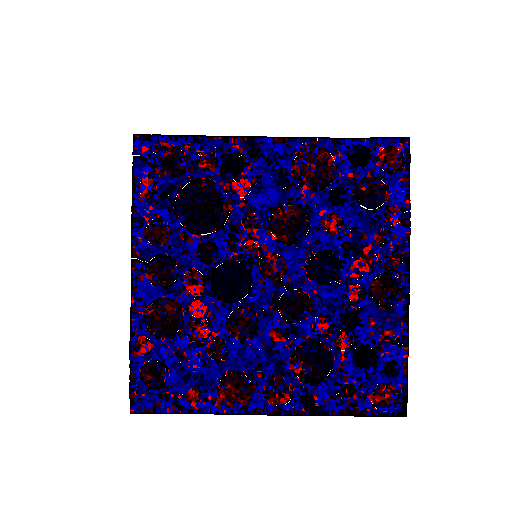
\includegraphics[width=1.0\linewidth]{Files/A30P75_3_IS/DEP50-STEP(014).png}
      \caption{Step 14}
      \end{subfigure}%
      %*******
      \begin{subfigure}{.25\textwidth}
        \centering
        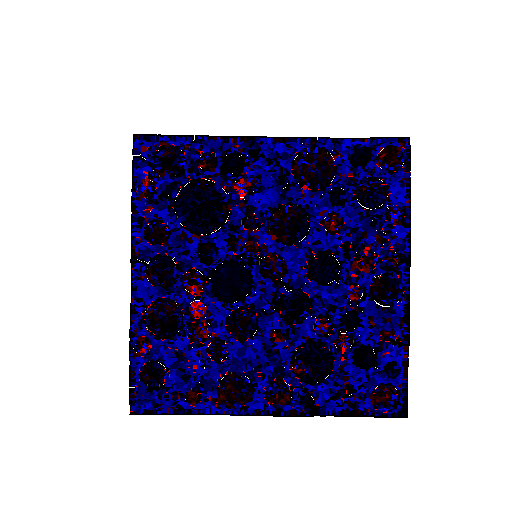
\includegraphics[width=1.0\linewidth]{Files/A30P75_3_IS/DEP50-STEP(015).png}
      \caption{Step 15}
      \end{subfigure}%
      %*******
      \begin{subfigure}{.25\textwidth}
        \centering
        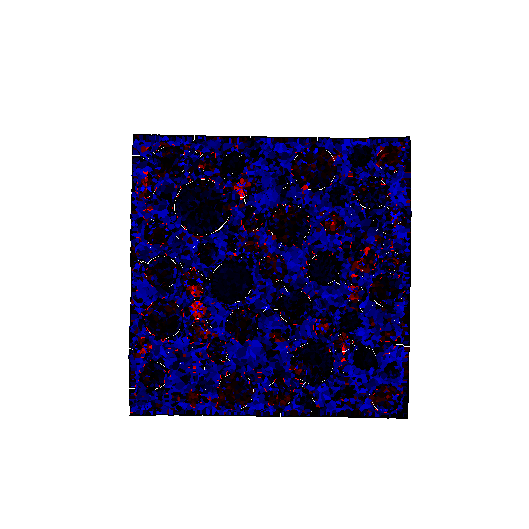
\includegraphics[width=1.0\linewidth]{Files/A30P75_3_IS/DEP50-STEP(016).png}
      \caption{Step 16}
      \end{subfigure}

      %*******
      %*******
      \begin{subfigure}{.25\textwidth}
        \centering
        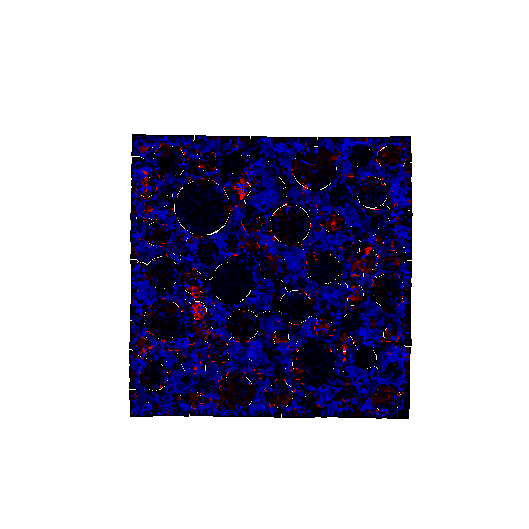
\includegraphics[width=1.0\linewidth]{Files//A30P75_3_IS/DEP50-STEP(017).png}
      \caption{Step 17}
      \end{subfigure}%
      %*******
      \begin{subfigure}{.25\textwidth}
        \centering
        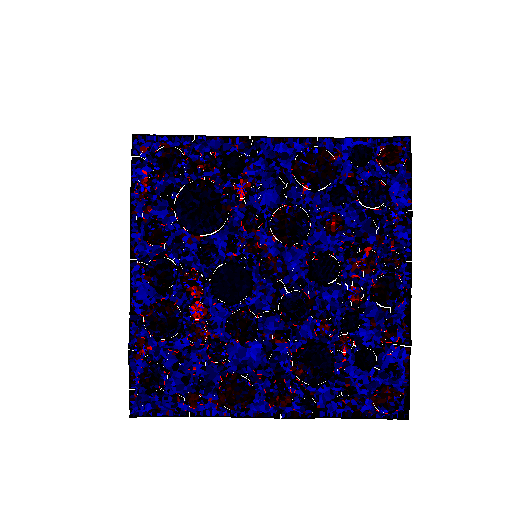
\includegraphics[width=1.0\linewidth]{Files/A30P75_3_IS/DEP50-STEP(018).png}
      \caption{Step 18}
      \end{subfigure}%
      %*******
      \begin{subfigure}{.25\textwidth}
        \centering
        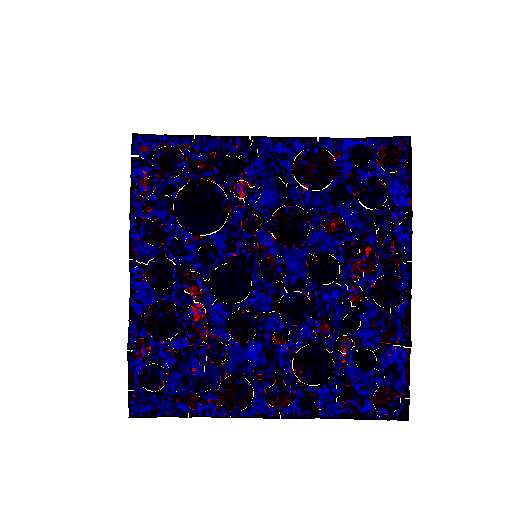
\includegraphics[width=1.0\linewidth]{Files/A30P75_3_IS/DEP50-STEP(019).png}
      \caption{Step 19}
      \end{subfigure}%
      %*******
      \begin{subfigure}{.25\textwidth}
        \centering
        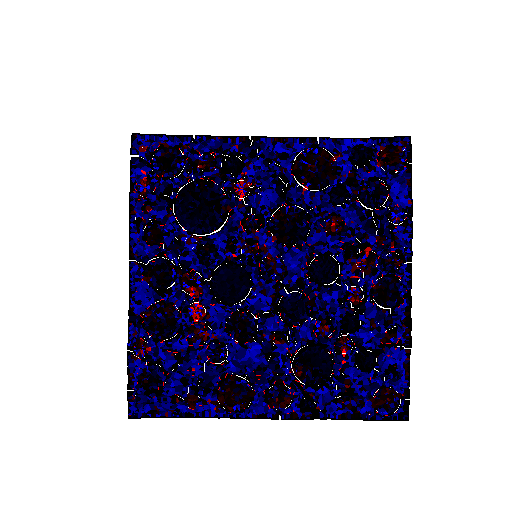
\includegraphics[width=1.0\linewidth]{Files/A30P75_3_IS/DEP50-STEP(020).png}
      \caption{Step 20}
      \end{subfigure}

      \begin{subfigure}{0.8\textwidth}
  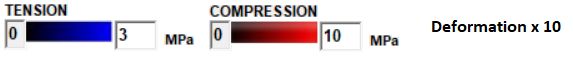
\includegraphics[width=0.8\linewidth]{Files/exp_3D/tagCS10.png}
\end{subfigure}%


  \caption{Internal Stress in Each Step for A30 P75 Case 3 (Deformation x 10)}
  \label{fig:ASR_A30P75_3_IS}
  \end{figure}

As can be seen in Figure \ref{fig:ASR_A30P75_3_IS} the internal stress from step 1 to 20, along with the increasing of giving initial strain, unbalanced force present in the concrete model, compressive stress (in red color) generated and distributed especially in coarse aggregates. Gradually crack generated around the aggregate, penetrated and finally linked between aggregates and reached surface of the model.

\begin{figure}[ht!]
\centering
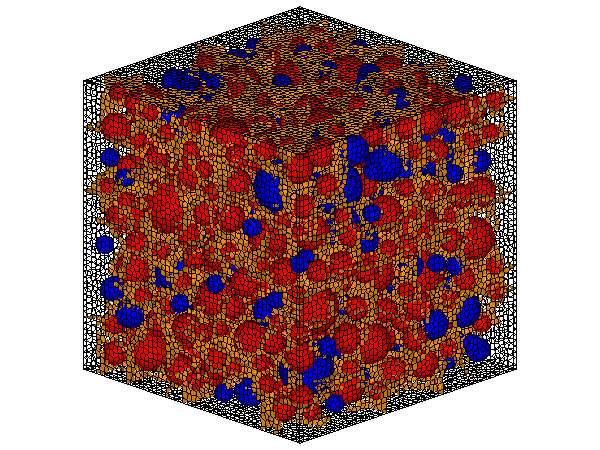
\includegraphics[width=.5\linewidth]{Files/exp_3D/ASR/A30P75_3_c.png}
  \caption{3D Inner Cracking larger than 0.03mm}
  \label{fig:A30P75_3_crack}
\end{figure}

In Figure \ref{fig:A30P75_3_crack} shows the inner crack distribution right after 20 steps of ASR expansion. The cracked interfaced which larger than 0.03mm are colored in orange, to present the distribution of internal crack three dimensionally. With 0.4223\% of one dimensional global expansion, cracks over 0.03mm are distributed relatively uniformed inside the model.

For analyzing the behavior of expansion caused by ASR numerically, cracked interfaces are summarised in different crack width scale, shown in Table \ref{table:A30P75_3_Cracks} and Figure \ref{A30P75CR_3}. The maximum crack width, in this case, is in range of 0.01-0.03mm, while most of the cracks are under 0.001mm. The ability of RBSM simulation in numerically analysis distribution of cracked interfaces gives us information that with difficulties to obtain in experimental tests. These numbers will be compared with simulations given different global expansion ratio, different aggregate consistent, even different mechanism.

\begin{table}[!h]
\centering
\begin{tabular}{ |p{4cm}|p{5cm}| }
\hline
 Crack Width [mm] &  Total Cracked Interfaces \\
 \hline\hline

   0.00000 - 0.00005 & 316744 \\
   0.00005 - 0.00010 & 286704 \\
   0.00010 - 0.00020 & 263943 \\
   0.00020 - 0.00050 & 234672 \\
   0.00050 - 0.00100 & 183238 \\
   0.00100 - 0.00300 & 131553 \\
   0.00300 - 0.01000 & 42432 \\
   0.01000 - 0.03000 & 275 \\
   0.03000 - 0.10000 & 0 \\
   0.1000+ & 0 \\

  \hline
  \end{tabular}
\caption{Crack Summarised by width}
\label{table:A30P75_3_Cracks}
\end{table}

\begin{figure}[ht!]
\centering
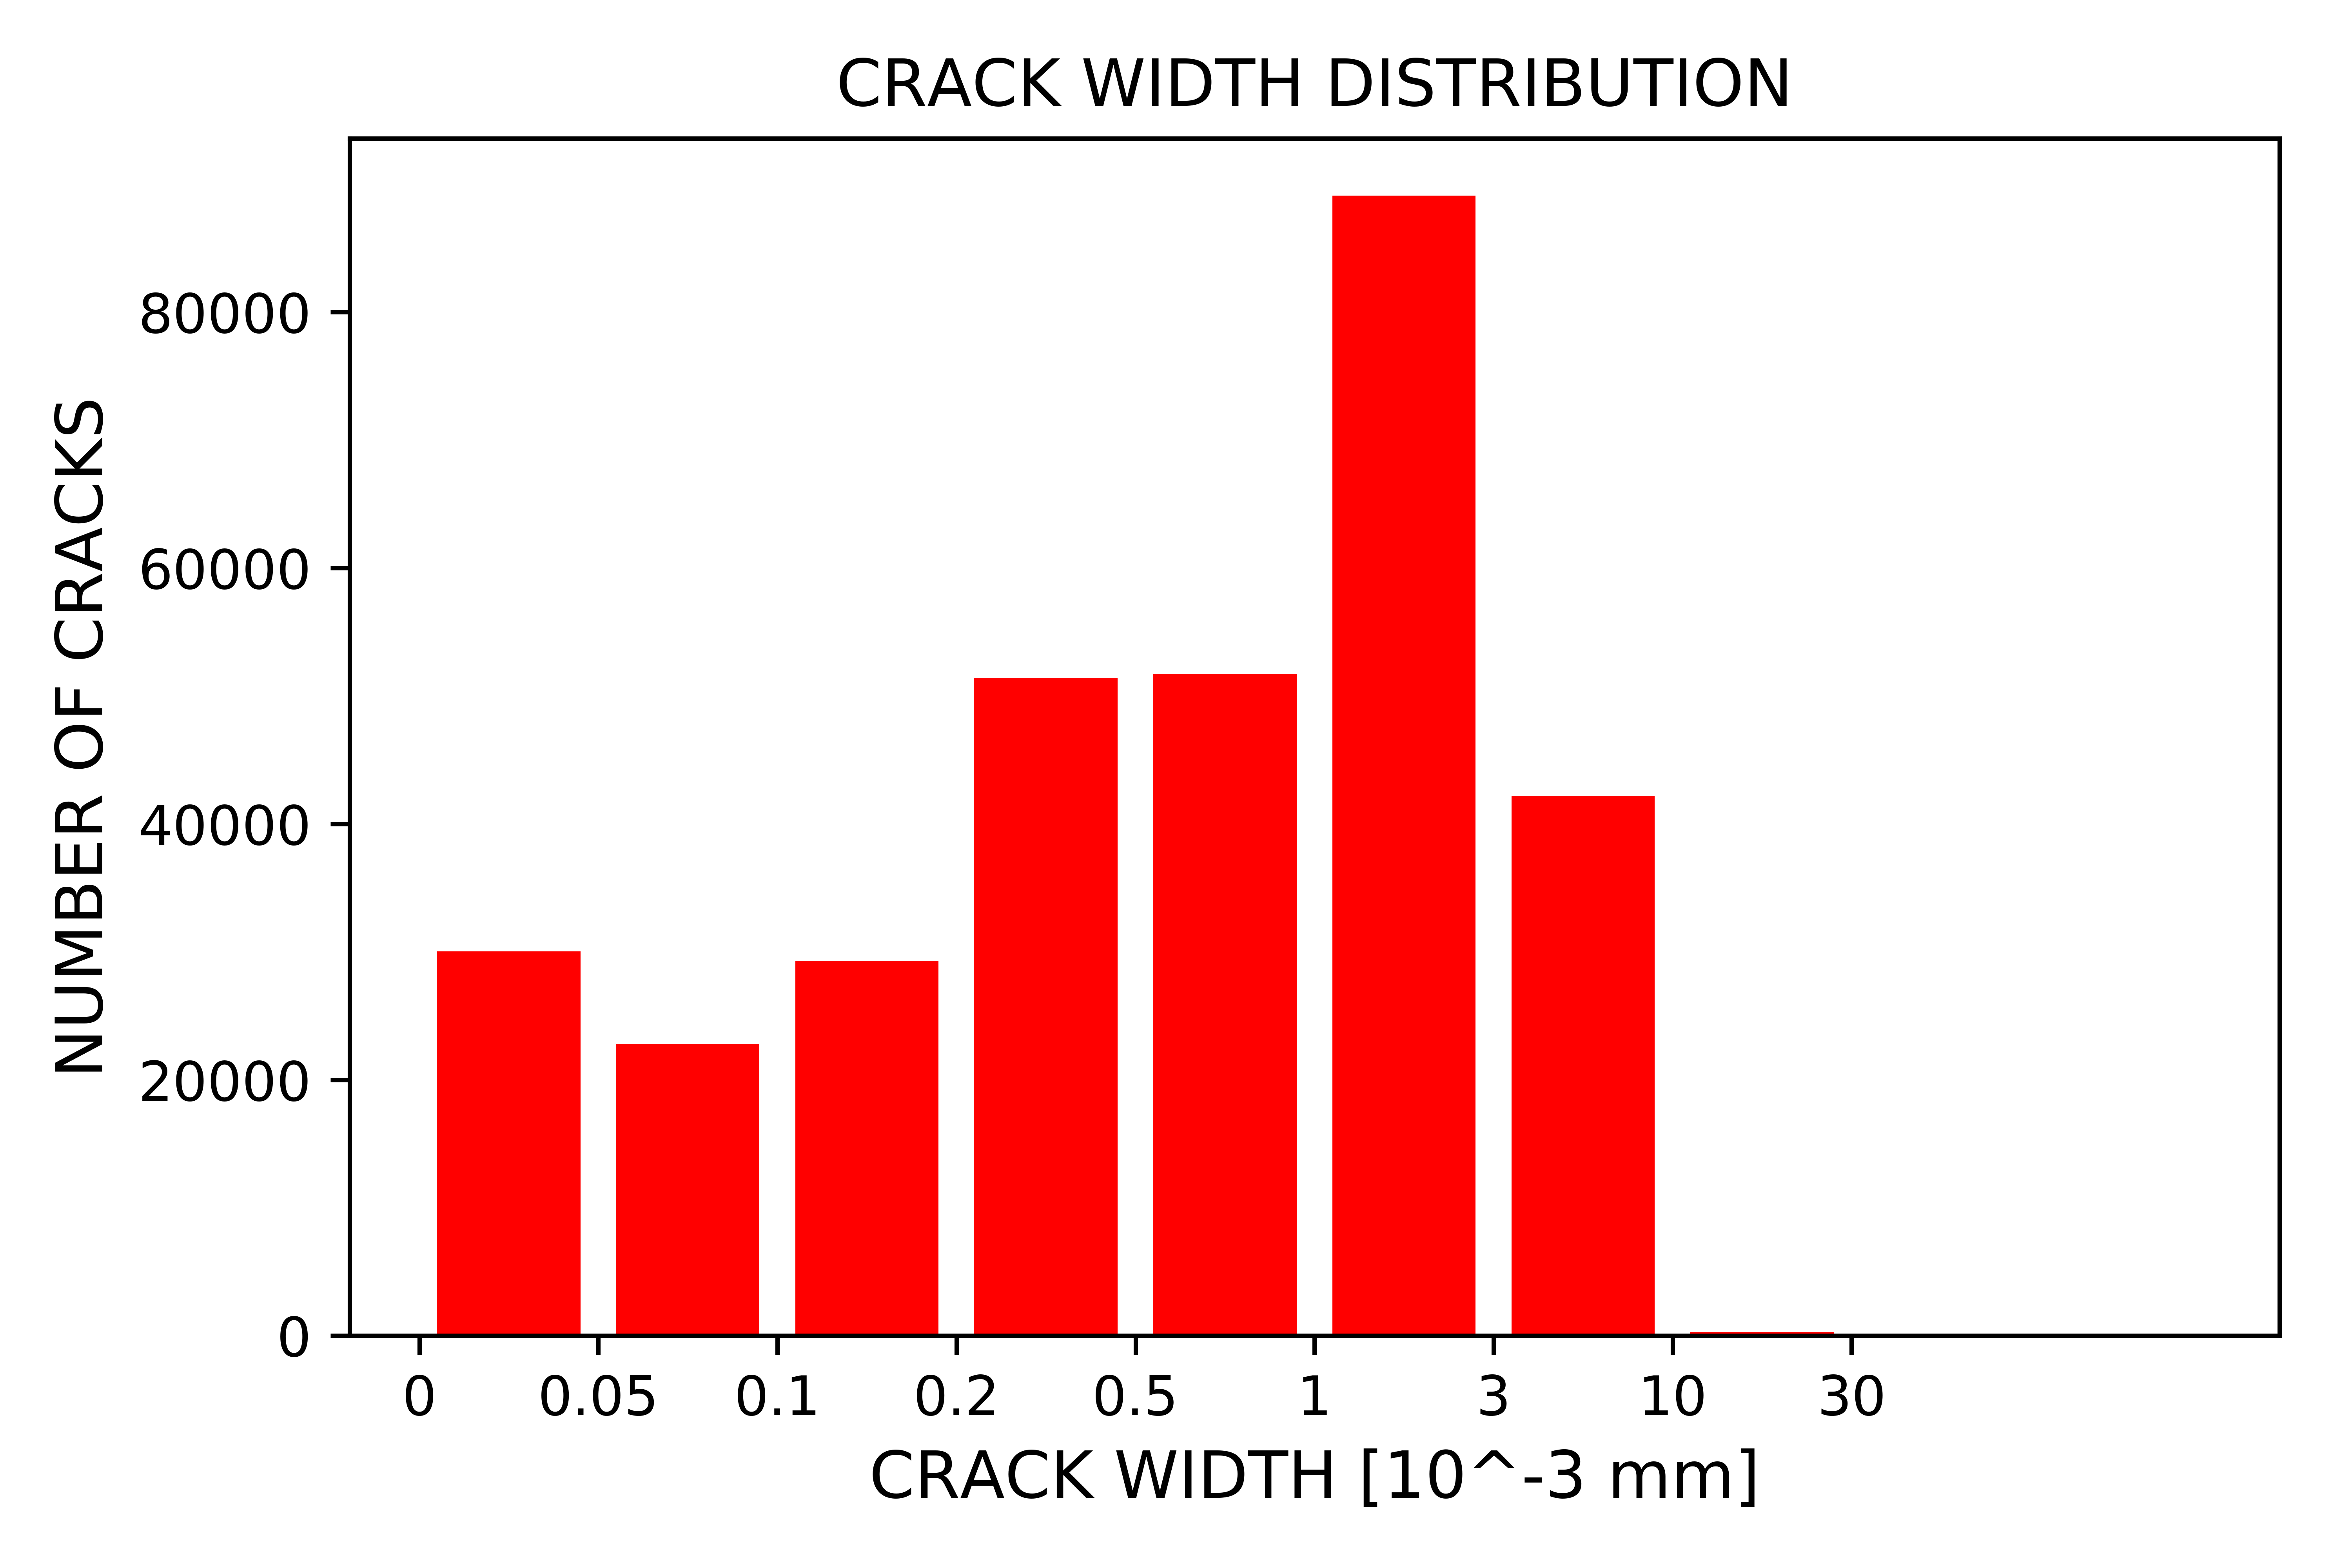
\includegraphics[width=.8\linewidth]{Files/interface/A30P75_3.png}
  \caption{Number of Cracked Interface vs. Expansion}
  \label{A30P75CR_3}
\end{figure}

In Figure \ref{fig:A30P75_3_crack}, inner cracking interfaces with over 0.03mm are colored in orange. From this illustration, it can be seen that the cracks are distributed relatively uninformed in the expanded model, which is co-insistent with the condition shown in the 2D inner section.
